% chapters/10/section-03.tex
\section{Heuristik dan Pengaruhnya}
\label{sec:heuristik}

Heuristik adalah jantung algoritma A*. Bagian ini membahas dua ukuran yang
dipakai pada bab ini dan mengukur pengaruhnya, sesuai indikator \ind{b}.

\subsection{Dua Ukuran Perkiraan Jarak}

Panel kanan Gambar~\ref{fig:peta-heuristik} memperlihatkan dua ukuran yang
paling sering dipakai, masing-masing beserta namanya.

\begin{itemize}
  \item \textbf{Jarak Manhattan}, yaitu jumlah selisih mendatar dan selisih
        tegak. Ukuran itu menyatakan banyaknya langkah terkecil yang diperlukan
        untuk berpindah pada peta yang hanya mengizinkan empat arah.
  \item \textbf{Jarak Euclidean}, yaitu jarak garis lurus antara kedua petak.
        Ukuran itu selalu lebih kecil atau sama dengan jarak Manhattan, sebab
        garis lurus adalah lintasan terpendek antara dua titik.
\end{itemize}

\subsection{Syarat agar Jalur Tetap Terpendek}

Sebuah heuristik boleh dipakai apabila ia \textbf{tidak pernah melebihkan}
jarak yang sebenarnya. Sifat itu disebut \istilah{admissible}.

Kedua ukuran di atas memenuhinya untuk gerak empat arah. Jarak Manhattan justru
tepat sama dengan jarak sebenarnya, sedangkan jarak Euclidean selalu lebih kecil
atau sama. Karena itu, keduanya menghasilkan jalur terpendek.

Sebaliknya, jarak Manhattan \textbf{tidak} memenuhi syarat itu pada peta yang
mengizinkan delapan arah, sebab perpindahan diagonal menempuh jarak sebenarnya
sebesar $\sqrt{2}$ sedangkan jarak Manhattan menghitungnya dua. Heuristik yang
melebihkan jarak dapat membuat A* memilih jalur yang bukan terpendek, walaupun
pencariannya menjadi lebih cepat. Pertukaran itu harus dipilih secara sadar.

\subsection{Hasil Pengukuran}

Program bab ini dapat menjalankan ketiga pilihan heuristik pada peta yang sama,
lalu membandingkan hasilnya. Pilihannya adalah \code{manhattan},
\code{euclidean}, dan \code{tanpa} yang berarti $h = 0$, yaitu Dijkstra.
Tabel~\ref{tab:perbandingan-heuristik} memuat hasilnya.

\begin{table}[htbp]
\centering
\caption{Perbandingan tiga heuristik pada satu peta yang sama}
\label{tab:perbandingan-heuristik}
{\setlength{\tabcolsep}{4pt}\footnotesize%
\begin{tabularx}{\textwidth}{@{}L{3.0cm} C{2.6cm} C{2.2cm} Y@{}}
\toprule
\headrow \textbf{Heuristik} & \textbf{Petak diperiksa} & \textbf{Biaya jalur} & \textbf{Keterangan} \\
\midrule
Manhattan & 274 petak & 50 &
Perkiraan tepat sama dengan jarak sebenarnya, sehingga pencarian paling
terarah. \\
\addlinespace
Euclidean & 353 petak & 50 &
Perkiraan lebih kecil daripada jarak sebenarnya, sehingga pencarian kurang
terarah dan lebih banyak petak diperiksa. \\
\addlinespace
Tanpa perkiraan & 437 petak & 50 &
Sama dengan algoritma Dijkstra: pencarian menyebar ke segala arah tanpa arah
tujuan. \\
\bottomrule
\end{tabularx}}
\tabsource{Pengukuran penulis pada peta bab ini, dengan panjang jalur 51 petak.
Angka pada komputer Anda akan sama, sebab pencariannya tidak bergantung pada
kecepatan komputer.}
\end{table}

Tiga hal dapat dibaca dari tabel tersebut.

\begin{enumerate}
  \item \textbf{Biaya jalurnya sama pada ketiganya}, yaitu 50. Ketiga
        heuristik itu tidak melebihkan jarak, sehingga ketiganya menghasilkan
        jalur terpendek. Inilah bukti optimalitas yang dijanjikan pada
        Bagian~\ref{sec:bfs-dijkstra-astar}.
  \item \textbf{Banyaknya petak yang diperiksa berbeda-beda.} Manhattan
        memeriksa paling sedikit, sedangkan Dijkstra memeriksa paling banyak,
        yaitu sekitar 1,6 kali lipat Manhattan. Perbedaan itu menyatakan
        besarnya manfaat arah tujuan.
  \item \textbf{Perbedaan itu menjadi jauh lebih besar pada peta yang lebih
        luas.} Pada peta bab ini yang berukuran 32 kali 20 petak, selisihnya
        163 petak. Pada peta yang berukuran sepuluh kali lipat, selisihnya
        bertambah jauh lebih besar daripada sepuluh kali lipat, sebab
        penyebaran Dijkstra tumbuh ke segala arah.
\end{enumerate}

\subsection{Melihat Perbedaannya pada Tangkapan Layar}

Angka pada tabel dapat lebih meyakinkan apabila disertai gambar.
Gambar~\ref{fig:pencarian-manhattan} dan
Gambar~\ref{fig:pencarian-dijkstra} memperlihatkan keadaan pencarian pada peta
yang sama, dengan heuristik yang berbeda.

\begin{figure}[htbp]
\centering
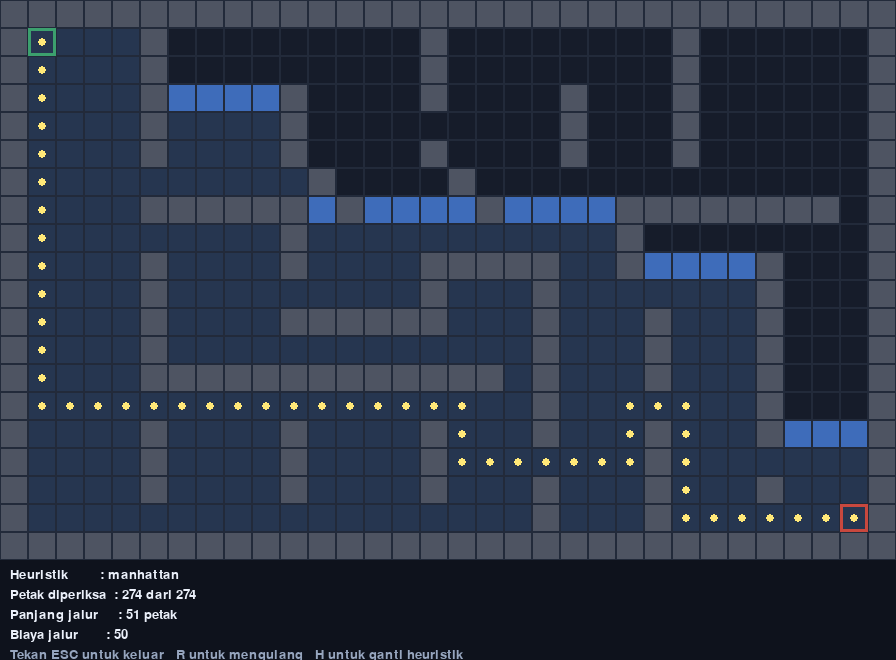
\includegraphics[width=0.86\textwidth]{figures/pencarian-manhattan.png}
\caption{Pencarian dengan heuristik Manhattan: 274 petak diperiksa}
\label{fig:pencarian-manhattan}
\end{figure}

\begin{figure}[htbp]
\centering
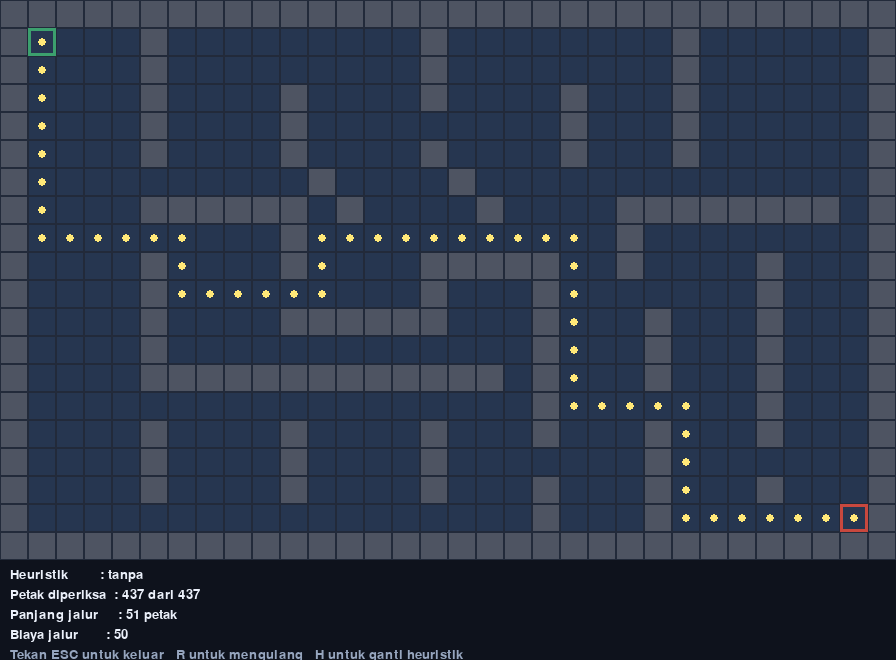
\includegraphics[width=0.86\textwidth]{figures/pencarian-dijkstra.png}
\caption{Pencarian Dijkstra tanpa perkiraan: 437 petak diperiksa}
\label{fig:pencarian-dijkstra}
\end{figure}

Pada kedua gambar, petak berwarna biru gelap adalah petak yang telah diperiksa,
petak biru terang adalah petak yang menunggu diperiksa, dan bulatan kuning
adalah jalur yang ditemukan. Jalur kuningnya sama persis pada
kedua gambar, tetapi luas daerah yang diperiksa jauh berbeda.

\begin{catatabox}
Kedua gambar itu bukan hiasan, melainkan hasil tangkapan layar dari program
yang Anda tulis sendiri, melalui pilihan \code{--simpan-gambar}. Kebiasaan
menyimpan gambar keadaan internal program---bukan hanya gambar permainannya---
sangat berguna ketika menyusun laporan praktikum dan laporan proyek akhir.
\end{catatabox}
